% Figure 1: Overall System Architecture (8 Modules, 3 Layers)
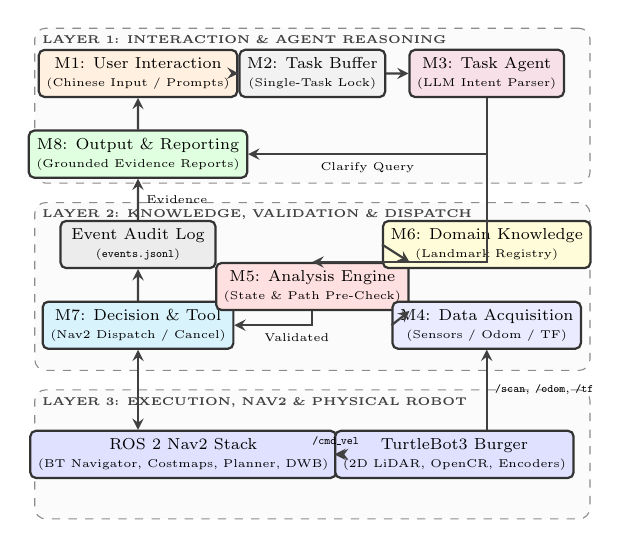
\begin{tikzpicture}[
    scale=0.82, every node/.style={transform shape},
    box/.style={rectangle, draw=black!80, fill=blue!5, thick, rounded corners=2pt, minimum width=2.3cm, minimum height=0.72cm, align=center, font=\scriptsize},
    layer/.style={rectangle, draw=black!45, dashed, fill=gray!3, rounded corners=4pt, inner sep=5pt},
    arr/.style={->, >=stealth, thick, draw=black!75},
    biarr/.style={<->, >=stealth, thick, draw=black!75},
    lbl/.style={font=\tiny\bfseries, text=black!75}
]

% ================= LAYER 1: INTERACTION & AGENT REASONING =================
\node[layer, minimum width=8.6cm, minimum height=2.4cm] (l1) at (0, 3.5) {};
\node[lbl, anchor=north west] at (l1.north west) {LAYER 1: INTERACTION \& AGENT REASONING};

\node[box, fill=orange!12, minimum width=2.4cm] (m1) at (-2.7, 4.0) {M1: User Interaction\\ \tiny (Chinese Input / Prompts)};
\node[box, fill=gray!10,   minimum width=2.2cm] (m2) at (0.0, 4.0)  {M2: Task Buffer\\ \tiny (Single-Task Lock)};
\node[box, fill=purple!12, minimum width=2.3cm] (m3) at (2.7, 4.0)  {M3: Task Agent\\ \tiny (LLM Intent Parser)};
\node[box, fill=green!12,  minimum width=2.4cm] (m8) at (-2.7, 2.75) {M8: Output \& Reporting\\ \tiny (Grounded Evidence Reports)};

\draw[arr] (m1) -- (m2);
\draw[arr] (m2) -- (m3);
\draw[arr] (m3.south) |- node[below, font=\tiny, pos=0.75]{Clarify Query} (m8.east);
\draw[arr] (m8) -- (m1);

% ================= LAYER 2: KNOWLEDGE, VALIDATION & DISPATCH =================
\node[layer, minimum width=8.6cm, minimum height=2.6cm] (l2) at (0, 0.7) {};
\node[lbl, anchor=north west] at (l2.north west) {LAYER 2: KNOWLEDGE, VALIDATION \& DISPATCH};

\node[box, fill=gray!15,   minimum width=2.4cm] (log) at (-2.7, 1.35) {Event Audit Log\\ \tiny (\texttt{events.jsonl})};
\node[box, fill=cyan!15,   minimum width=2.4cm] (m7)  at (-2.7, 0.1)  {M7: Decision \& Tool\\ \tiny (Nav2 Dispatch / Cancel)};
\node[box, fill=red!12,    minimum width=2.4cm] (m5)  at (0.0, 0.7)   {M5: Analysis Engine\\ \tiny (State \& Path Pre-Check)};
\node[box, fill=yellow!15, minimum width=2.4cm] (m6)  at (2.7, 1.35)  {M6: Domain Knowledge\\ \tiny (Landmark Registry)};
\node[box, fill=blue!8,    minimum width=2.4cm] (m4)  at (2.7, 0.1)   {M4: Data Acquisition\\ \tiny (Sensors / Odom / TF)};

% Layer 2 intra-flows
\draw[arr] (m3.south) |- (m5.north);
\draw[arr] (m6.west) -- (m5.north east);
\draw[arr] (m4.west) -- (m5.south east);
\draw[arr] (m5.south) |- node[below, font=\tiny, pos=0.6]{Validated} (m7.east);
\draw[arr] (m7) -- (log);
\draw[arr] (log) -- node[right, font=\tiny]{Evidence} (m8);

% ================= LAYER 3: EXECUTION, NAV2 & PHYSICAL ROBOT =================
\node[layer, minimum width=8.6cm, minimum height=2.0cm] (l3) at (0, -1.9) {};
\node[lbl, anchor=north west] at (l3.north west) {LAYER 3: EXECUTION, NAV2 \& PHYSICAL ROBOT};

\node[box, fill=blue!12, minimum width=3.4cm] (nav) at (-2.0, -1.9) {ROS 2 Nav2 Stack\\ \tiny (BT Navigator, Costmaps, Planner, DWB)};
\node[box, fill=blue!12, minimum width=3.0cm] (tb3) at (2.2, -1.9)  {TurtleBot3 Burger\\ \tiny (2D LiDAR, OpenCR, Encoders)};

% Inter-layer execution connections
\draw[biarr] (m7.south) -- (m7.south |- nav.north);
\draw[biarr] (nav) -- node[above, font=\tiny]{\texttt{/cmd\_vel}} (tb3);
\draw[arr]   (tb3.north -| m4.south) -- node[right, font=\tiny]{\texttt{/scan}, \texttt{/odom}, \texttt{/tf}} (m4.south);

\end{tikzpicture}
